\section{Incremental Filtering and Embedding}
\label{sect:incremental-filtering-and-embedding}

The incremental filtering and embedding phase continues propagating the changes and translates changes of the cluster graph to changes of its filtered graph embedding: it takes a cluster graph, a sequence of operations to be applied to the cluster graph, and the embedded filtered graph of the cluster graph and outputs a sequence of operations that, when applied to the embedded filter graph, makes it an embedded filter graph of the cluster graph with the operations applied.

\begin{figure}[H]
	\centering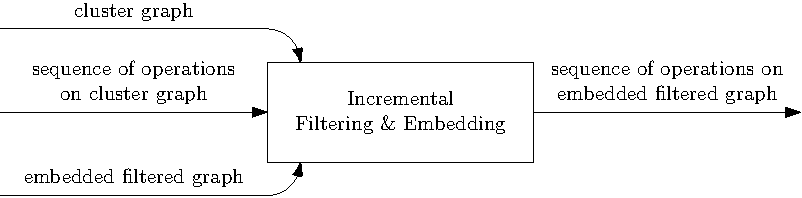
\includegraphics[width=0.9\textwidth]{Resources/DynamicPipeline-IncrementalFilteringAndEmbedding.pdf}
	\caption{Input and output of the incremental filtering and embedding phase.}
	\label{fig:dynamic-pipeline-incremental-filtering-and-embedding}
\end{figure}

The pipeline supports the following operations:
%Supported operations on embedded filtered graph:
%
\begin{itemize}
	\item \textbf{Change vertex or edge weight:}
	\item \textbf{Add vertex in an internal face:} with arbitrary weight inside an inner face (and connect it to the three vertices of the triangle)
	\item \textbf{Add vertex in outer face:} adjacent to 2 or more vertices on outer face that lie on simple path
	\item \textbf{Remove internal vertex:} of degree 3
	\item \textbf{Add edge on outer face:}
	\item \textbf{Remove edge on outer face:} without violating 2-connectedness and internal triangulatedness
	\item \textbf{Flip internal edge:}
\end{itemize}
